% !TeX spellcheck = en_US
 
\chapter{Tools} %Das ist nur ein Arbeitstitel
\section{Template}
\subsection{Toolname}
\label{Toolname} % to refernce in the document
Introduction Text with all infos about contributors and installation Process
\subsubsection{Appearance}%Only for Visual tools
Description of the tool front-end with a Screen shot of the homepage/Dashboard
\subsubsection{Performance}
Quick analysis of the Performance (CPU/RAM usage during the test)
\subsubsection{Interoperability}
Which tools are listed to work with the tool/Which tools are test to work with the tool
\subsubsection{Conclusion}
A Quick Pro/Con of the tool and in which environment its best to use
\section{Installed Tools}%Arbeitstitel
\subsection{Searchlight (Icinga)}
\label{searchlight}
As in the Section Icinga \ref{Icinga} described, we were not able to find a pure installation of Icinga for a cluster so we tried to install Searchlight as a backup plan.
Searchlight is a tool from the AppsCode Inc. (\url{https://appscode.com/},18.12.2017) which is a company located in San Leandro Californian.
\\
When first trying this over the yaml File we resived errors over the Kubernetes Cluster. There it says the tools is not able to bind the Port 8443. We could not figure out wich Apllication is using the port but as we tried to install the app on a fresh cluster VM it turns out the yaml deployment is working fine.
\subsubsection{Appearance}
%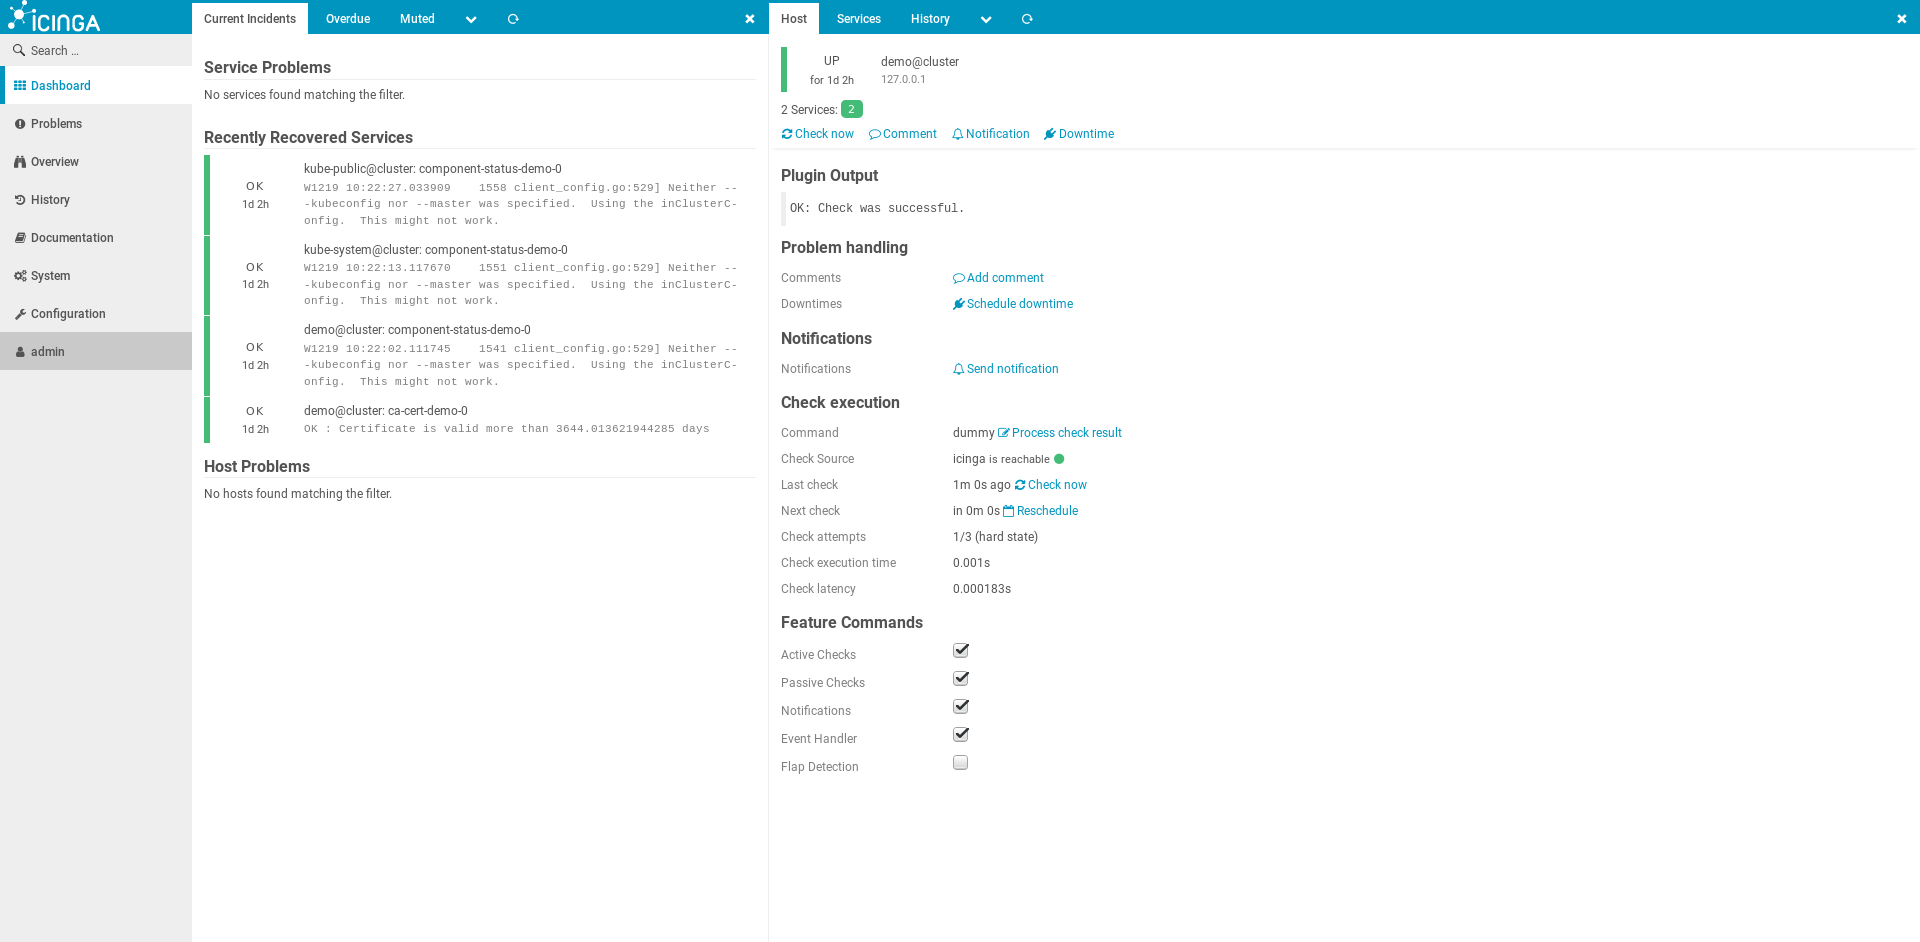
\includegraphics[width=1\linewidth]{Bilder/Searchlight_Icinga}\\
Icinga/Searchlight comes in a  discreet blue/withe coloring. On the Dashboard which represents the homepage of the application an overview of the implemented alerts is shown. The alerts will be Colored with Green/Yellow/Red for OK/Warning/Error, so its easy to see appearing problems. The rest of the option as History and Configurations is located at the sidebar. 
\subsubsection{Performance}
In our VM deployment the applications has allocated 160MB of RAM under Load. The Application it self is Running very smooth even on low Power Systems. As we deployed some alerts we noticed that it took about 30 seconds to validate the alert and get a first status from the system. After that pending status run Smoothly and even checks on a 30 seconds bases were no Problem for the System.




\section{Failed Tools}%Ebenfalls nur ein arbeitstitel
In the Process of Developing and Evaluating the APM we Discoverd a bunch of Tools that we were not able to install even that they clamed to be optimized to work on Kubernetes .
In this Paragraph all the tools we wanted to include in our Report but doesn't are mentioned with a quick description of the Failure.
\subsection{Graphite}
Graphite is mainly for storing and Graphing data and metrics, but brings also tools that are able to collect these Metrics from the system. By the Developer it self there is no Kubernetes installation Provide but there are diverse approaches by third party members to make it runnable on a Cluster. We have tested the Repository from nanit\\(\url{ https://github.com/nanit/kubernetes-graphite-cluster},11.12.2017) to get Graphite running with StatsD (\url{https://github.com/etsy/statsd.git},11.12.2017) as a metric collection tool. The Repo doesn't provide a yaml file by it self to install all the tools. The instruction leads the user to export some Variables needed for the installation. After that a deploy command is provided that pulls the docker repo and than installs it with kubectl on the Cluster. As we tried to execute this command a fail was thrown, The Node Replicas were empty, so no further commands are executable. As we were not able to install the tool on multiple Kubernetes Clusters, we installed the tool as on the Webside advertised on a Ubuntu System directly. With this installation of Graphit a time-series Data,an Monitoring and an Alerting tool is included. On the test System the Monitoring System gave values that differs from the Linux intern monitoring in values like Cpu usage or RAM. As a Solution to all this Difficulties we decided to not perform further test on the tool.

\subsection{Icinga}
\label{Icinga}
As we tried to install Icinga as we found out that there was no direct support from Incinga for Kubernetes. As our Study only describes the actual state without trying to add somthing we decidet not to try an compile Icinga into Kuberntes on oure own. Later we found out there is a third party Software called searchlight \ref{searchlight}. Its provided by appscode on github.
 